%!TEX root = ../template.tex
%%%%%%%%%%%%%%%%%%%%%%%%%%%%%%%%%%%%%%%%%%%%%%%%%%%%%%%%%%%%%%%%%%%
%% chapter1.tex
%% NOVA thesis document file
%%
%% Chapter with introduction
%%%%%%%%%%%%%%%%%%%%%%%%%%%%%%%%%%%%%%%%%%%%%%%%%%%%%%%%%%%%%%%%%%%

\typeout{NT FILE chapter1.tex}%

\chapter{State of the Art}
\label{cha:state_of_the_ art}

\prependtographicspath{{Chapters/Figures/Covers/}}

% epigraph configuration
\epigraphfontsize{\small\itshape}
\setlength\epigraphwidth{12.5cm}
\setlength\epigraphrule{0pt}

This chapter establishes the theoretical framework for the development of a distributed controller communication tool. It begins with an exploration of Petri nets, which are foundational in modeling the interactions and behavior of distributed systems. Following this, the chapter discusses \gls{gals} (Globally Asynchronous, Locally Synchronous) communication technologies, highlighting their significance in enabling efficient and reliable communication within distributed systems. The discussion then examines various communication protocols, including \gls{i2c},  \gls{spi}, \gls{uart}, RS-485 and \gls{fifo} with handshake, evaluating their suitability and ensuring effective communication within the distributed \gls{iopt} controller system .Finally, the chapter introduces the \gls{iopt}-Tools environment, focusing on its role in supporting the design and development of the distributed controller communication tool.

\section{Petri Nets}
\label{sec:petri_nets}


\subsection{History}
\label{subsec:history}
The German computer scientist Carl Adam Petri formalized the concept of  Petri nets, as a formalism for modeling distributed and concurrent systems, in his 1962 PhD dissertation, \emph{Kommunikation mit Automaten}, at the Technical University of Darmstadt~\cite{petri1962}, in the following years, the theoretical foundations of Petri nets were strengthened by seminal results on decision problems such as reachability and liveness~\cite{murata}, while the annual International Conference on Applications and Theory of Petri Nets and Concurrency provided a forum to advance both theory and practice~\cite{ICPN1980}, firmly establishing Petri nets as a formal graphical language for discrete‐event and concurrent systems modeling~\cite{WikiPetriNet2025}.


In subsequent decades, the theoretical foundations of Petri nets were strengthened by seminal results on decision problems such as reachability and liveness~\cite{murata}, while the establishment of the International Conference on Applications and Theory of Petri Nets and Concurrency created an annual forum to advance both theory and practice~\cite{ICPN1980}, firmly establishing Petri nets as a formal graphical language for discrete‐event and concurrent systems modeling~\cite{WikiPetriNet2025}.

\subsection{Definition}
\label{subsec:definition}


Petri nets, over the years, have been developed and adapted to better suit different applications,  Colored Petri Nets (CPNs), Timed Petri Nets, Hierarchical Petri Nets, Input-Output Place-Transition (\gls{iopt}), among others were introduced to better meet these needs. 


To manage this diversity, the term \textbf{Place/Transition net (P/T net)} was established as the standard name for the classical formalism, a standardization heavily influenced by seminal works such as Murata's~\cite{murata}. This P/T net serves as the foundational model from which the advanced types mentioned above are derived from. Essentially, every advanced Petri net is an extension of the classical P/T net, inheriting its fundamental concepts of places, transitions, and firing rules. A firm grasp of the P/T net definition is therefore a prerequisite for understanding its more complex variants.

Place/Transition nets are a bipartite directed‐graph formalism comprising primitive elements, \emph{places} (depicted as circles), \emph{transitions} (depicted as bars) and \emph{Arcs} (depicted as arrows), and \emph{tokens} that reside in places to represent system state (see Figure~\ref{fig:petri_diagrama}). The minimality of these primitives enables the construction of richer constructs (e.g., forks, joins) while preserving analytical tractability~\cite{50-years}. Semantically, places model local conditions or resources and transitions denote events whose firing consumes and produces tokens, thereby capturing concurrency, synchronization, conflict and choice within a unified mathematical framework~\cite{50-years}. 

Graphically, P/T nets serve as intuitive visual‐communication aids for stakeholders, such as clients, manufacturers and users, supporting model comprehension and system specification~\cite{pn-Wolfgang}.

 Mathematically, they admit formalisms like state equations and algebraic invariants for rigorous analysis; however, there is a critical tradeoff between modeling generality and analysis capability, often necessitating application‐specific restrictions or tool support for simulation and verification~\cite{murata}.This inherent complexity, where Petri-net-based models can become too large for analysis even for a modest-size system, is mitigated in the \gls{iopt}-Tools environment through its support for hierarchical modeling and decomposition into independent sub-models, which aids in managing the complexity for distributed systems.


\begin{figure}[htbp]
  \centering
  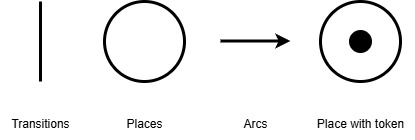
\includegraphics[width=0.6\textwidth]{Chapters/Figures/petri_image.jpg}
  \caption{Petri net elements.}
  \label{fig:petri_diagrama}
\end{figure}



The formal definition of a P/T net states that a Petri net \( \gls{pn} \) is defined as the tuple (meaning they cannot be modified once created) \( \gls{pn} = (P, T, F, W, M_0) \)~\cite{murata}, where:


\begin{itemize}
    \item \( P = \{ p_1, p_2, p_3, \ldots, p_m \} \) is the set of \( m \) places;
    \item \( T = \{ t_1, t_2, t_3, \ldots, t_n \} \) is the set of \( n \) transitions;
    \item \( F \subseteq (P \times T) \cup (T \times P) \) is the set of arcs representing the flow relation;
    \item \( W : F \to \{1,2,3,\ldots\} \) is the arc weight function;
    \item \( M_0 : P \to \{0,1,2,3,\ldots\} \) is the initial marking;
    \item \( P \cap T = \emptyset \) and \( P \cup T \neq \emptyset \).
\end{itemize}

A Petri net structure \( N = (P, T, F, W) \) without an initial marking is denoted by \( N \) and a Petri net with an initial marking is denoted by \( (N, M_0) \).


Figure~\ref{fig:petrinet} presents a Place/Transition net that models the execution and synchronization of two parallel processes. The model demonstrates a classic fork-join structure, where concurrent tasks are initiated by transition $T_0$ and must both be completed before synchronizing at transition $T_3$ to continue the cycle.


\begin{figure}[htbp]
  \centering
  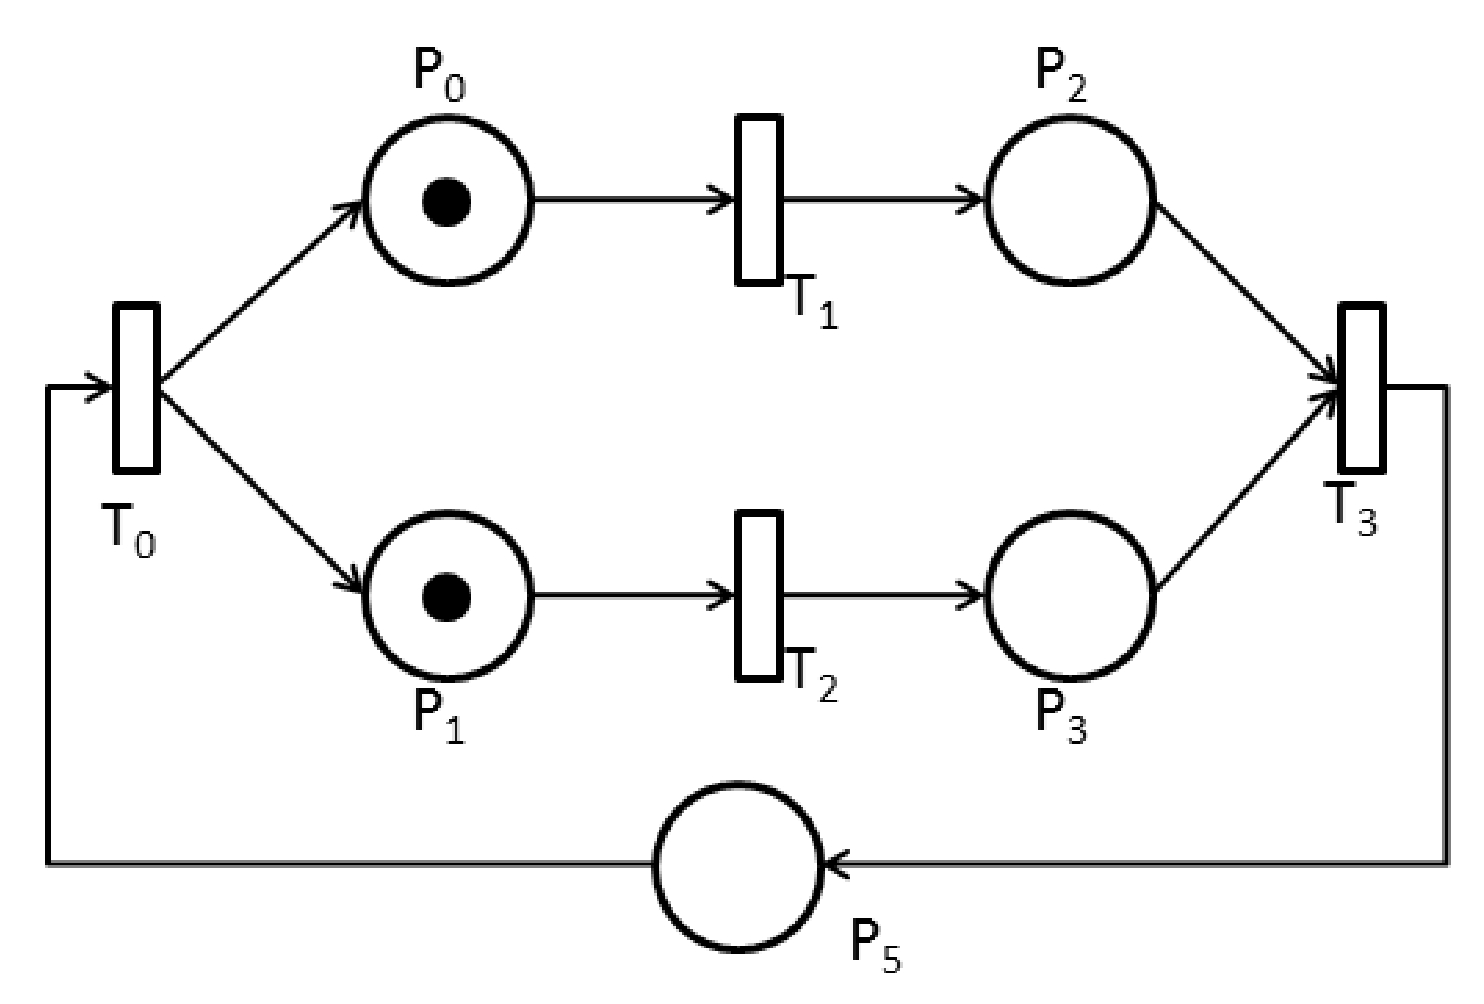
\includegraphics[width=0.6\textwidth]{Chapters/Figures/petriNetExemplo.jpg}
  \caption{Example of Place/Transition net.}
  \label{fig:petrinet}
\end{figure}

\section{\emph{Input-Output Place-Transition} Petri Nets}
\label{sec:iopt_petri_nets}


The \textbf{\gls{iopt} Petri Nets} were created to model controllers interacting with external environments through the use of (\gls{io}) interfaces\cite{iopttools}. They are considered \emph{non-autonomous}  where non-autonomous means that external signals can enable or disable transitions \cite{2015gomes}. The incorporation of inputs and output signals in Petri nets enables precise representation of the interactions between a controller and its external environment, therefore enabling its applicability in real-world environments  and making them particularly useful in automation and embedded systems\cite{iopttools}.


The \gls{iopt} framework can be defined as a tuple of input signals (IS), input events (IE), output signals (OS), and output events (OE). This design ensures the synchronization of the modeled control logic with the external environment \cite{iopttools}. The introduction of priority attributes for transitions and the inclusion of test arcs represent notable advancements over earlier versions of \gls{iopt} nets, such as those described in previous works in~\cite{barros2004} and~\cite{bg2005}. The introduction of prioritization allows for effective conflict resolution among transitions, while test arcs facilitate the implementation of fair arbitration mechanisms~\cite{conflict}.

Furthermore, the \gls{iopt} framework incorporates features such as time domains and communication channels, which support the modeling of networked controllers and globally-asynchronous locally-synchronous (\gls{gals}) systems. Its metamodel complies with the Petri Net Markup Language (\gls{pnml}) and extends it with Ecore-based representations to capture \gls{io}, timing, and communication aspects~\cite{iopttools}.


\begin{figure}[htbp]
  \centering
  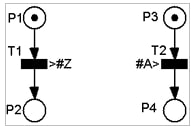
\includegraphics[width=0.6\textwidth]{Chapters/Figures/petrisplit.jpg}
  \caption{Example of IOPT Petri net.}
  \label{fig:petrisplit}
\end{figure}


Figure~\ref{fig:petrisplit} presents two Petri nets where transitions are made with communication actions (>\#Z on $T_1$ and \#A> on $T_2$). The figure demonstrates how locally asynchronous components achieve global synchrony. Structurally, the two sub-nets are independent, as the enabling of $T_1$ and $T_2$ depends only on their local markings but a transition can only fire if a complementary input/output action occurs simultaneously in its environment. In the state shown, although both transitions are locally enabled, they cannot synchronize with each other as their communication actions do not match; each must await a corresponding partner.



\subsection{IOPT Net Composition and Decomposition}
\label{sub:net_addicion}

Net Composition and Decomposition are fundamental operations in the \gls{iopt} Petri nets framework, they form the foundation for its adaptability in embedded and distributed systems.The combination and decomposition of two \gls{iopt} nets through synchronized transitions and shared places preserve the input/output (\gls{io}) signal dependencies~\cite{add1}.

\begin{itemize}
    \item \textbf{Net Composition: }     
As the term suggests, net composition functions as a composition operator that integrates two \gls{iopt} net modules into a larger model, thereby facilitating the reuse of pre-validated components. Comparable to additive compositionality~\cite{add2}, this operation transforms submodels into coherent systems while preserving semantic consistency through synchronized transitions and shared places, which maintain the dependencies of input/output (\gls{io}) signals~\cite{add1}.
\end{itemize}

\begin{itemize}
    \item \textbf{Net Decomposition (or Net Splitting): }     
    
Net Decomposition, or net splitting,  is a formal operation designed to divide Petri net models into a set of smaller, concurrent sub-models.The primary goal is to transform a centralized system specification into distributed components that can be independently implemented on various platforms, such as separate hardware controllers or software processes~\cite{co-design}. The use of net splitting creates smaller and more manageable systems, supporting modular design approaches and allowing for incremental development and analysis~\cite{Barrosadd}.

In net splitting operations, it is essential to identify and validate the nodes, known as the \emph{cutting set}, where the model should be broken. The validity of a cutting set is determined by adhering to the following rules introduced in ~\cite{splitting}:

\begin{enumerate}
    \item \textbf{Rule 1} - Splitting at a Place: This rule is invoked when the cutting node is a place. The fundamental precondition is that after the conceptual removal of the place, its pre-set (input transitions) and post-set (output transitions) are separated into different components.
    \item \textbf{Rule 2} - Splitting at a Transition with Single-Component Input: If a transition is the cutting node and all its input places belong to what will become a single component, the transition is kept in that "master" component. A copy of the transition is then placed in the component(s) containing the output places.
    \item\textbf{ Rule 3} - Splitting at a Transition with Multi-Component Input: If a cutting transition has input places that will belong to different components after the split, one component is designated as the "master." This master component receives the original transition and copies of the input places (and their preceding transitions) from the other components. The other components receive a copy of the cutting transition.
\end{enumerate}

To maintain behavioral consistency immediately after the split, the operation relies on synchronous communication channels ~\cite{splitting}, ~\cite{co-design}. When a node is split, the original and its copies are linked in a "synchrony set" or "synchrony group" ~\cite{co-design}. One transition in the set is designated as the "master" and the others as "slaves" ~\cite{splitting}, ~\cite{co-design}. Semantically, all transitions in a synchrony set are intended to fire simultaneously, as if they were a single fused transition ~\cite{splitting}. This ensures that, at the model level, the set of sub-models is behaviorally equivalent or similar to the original, monolithic net ~\cite{splitting}, ~\cite{co-design}.

\end{itemize}



\section{GALS}
\label{sec:gals}


The increasing complexity of embedded and distributed systems necessitates modeling approaches that can effectively handle concurrency, modularity, and varying timing constraints. \gls{gals} architectures address these needs by allowing system components to operate synchronously within themselves while communicating asynchronously with other components. When integrated into the \gls{iopt} Petri net framework, \gls{gals} architectures enable a structured and scalable approach to system design and verification.

In \gls{gals} (Globally Asynchronous, Locally Synchronous) systems, each local component operates synchronously with respect to its own local clock, which governs its state evolution. However, since each component resides in a distinct clock domain, the overall system exhibits asynchronous behavior. Inter-component communication can be facilitated through asynchronous wrappers, such as those proposed in~\cite{galsborman}.


An extension of \gls{gals} systems applied to \gls{iopt} models is presented in~\cite{galsactd}, where the author introduces an attribute that specifies the Time Domain (\gls{td}) of each node within the \gls{iopt} Petri net, including both places and transitions. This attribute enables the association of each node with a specific hardware or logical component, thereby facilitating modular and time-partitioned system design.
To support communication between components operating in different time domains, the model incorporates the concept of \gls{ac}. An \gls{ac} connects two transitions that belong to distinct time domains, for example, one acting as the master, responsible for sending events, and the other as the slave, which receives them. These events are transmitted across the \gls{ac}, enabling coordinated yet asynchronous interaction between independently clocked components.


An \gls{iopt} Petri net extended with Time Domains and Asynchronous Channels can be formally defined as follows:

\begin{equation}
\text{IOPT\_GALS} = (\text{IOPT}, \text{ACs}, \text{TDs})
\end{equation}

where:
\begin{enumerate}
    \item \textbf{IOPT} denotes an \gls{iopt} Petri net, defined as in~\cite{iopttools};
    \item \textbf{ACs} is the set of asynchronous channels;
    \item \textbf{TDs} is the set of time domains.
\end{enumerate}

An \gls{iopt} net is formally defined as:
\begin{equation}
\text{IOPT} = (P, T, A, TA, M, weight_T, weight_P, priority, isg, ie, oe, osc)
\end{equation}

The following constraints further define the \gls{iopt}-\gls{gals} structure:

\begin{equation}
ACs \subseteq T \times T
\end{equation}

\begin{equation}
t_s \times t_m \subseteq ACs
\end{equation}

\begin{equation}
TDs = TDs_p \cup TDs_t \cup TDs_{ac}
\end{equation}

\noindent where \( t_m \) and \( t_s \) denote the master and slave transitions, respectively, such that:
\[
t_m \in T, \quad t_s \in T, \quad t_m \neq t_s
\]

\noindent The mapping functions are defined as:
\[
TDs_p : P \rightarrow \text{IN}, \quad TDs_t : T \rightarrow \text{IN}, \quad TDs_{ac} : ACs \rightarrow \text{IN}
\]



The integration of \gls{gals} into \gls{iopt} Petri nets involves decomposing a global system model into locally synchronous modules that communicate asynchronously. This decomposition creates \gls{td} and \gls{ac}, it facilitates modular design, enabling each module to operate at its own pace without the need for global synchronization, thus improving scalability and flexibility \cite{galsactd}.




Figure~\ref{fig:petrigals} illustrates an example of a \gls{gals} system. The model depicts two distinct time domains: one on the left side (\( TD_1 \)) and another on the right side (\( TD_2 \)). Positioned between them is an asynchronous channel (\gls{ac}), which facilitates communication across time domains. 

All elements on the left side operate synchronously within \( TD_1 \), while those on the right side operate synchronously within \( TD_2 \). Components sharing the same time domain communicate synchronously. However, communication between components in \( TD_1 \) and \( TD_2 \) is asynchronous and is mediated by the \gls{ac}, which is associated with its own independent time domain.




\begin{figure}[htbp]
  \centering
  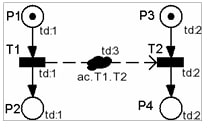
\includegraphics[width=0.6\textwidth]{Chapters/Figures/petrigals.jpg}
  \caption{Example of Petri net with GALS system.}
  \label{fig:petrigals}
\end{figure}


%%%%%%%%%%%%%%
%%%%%%%%%%%%%%
%%%%%%%%%%%%%%
%%%%%%%%%%%%%%
%%%%%%%%%%%%%%
%
%
%
%
%
%%%%%%%%%%%%%%
%%%%%%%%%%%%%%
%%%%%%%%%%%%%%
%%%%%%%%%%%%%%
%%%%%%%%%%%%%%

\section{Communication support technologies}
\label{sec:communication_support_technologies}

In this section, various communication technologies utilised within Globally Asynchronous Locally Synchronous (\gls{gals}) systems are examined. The analysis focuses on their design considerations, performance trade-offs, and integration challenges. By providing a comprehensive overview of these mechanisms, the chapter aims to equip readers with the knowledge necessary to navigate the complexities of modern integrated circuit development and to harness the benefits of \gls{gals} architectures for optimised system performance and reliability.


\subsection{I\textsuperscript{2}C}
\label{subsub:i2c}

The I\textsuperscript{2}C  (Inter-Integrated Circuit) protocol is described as a multi-master, serial, and single-ended bus that requires only two lines for communication: the clock line (SCL) for synchronization and the data line (SDA) for transmitting information. This simplicity is underscored by the minimal hardware requirements, just three connections (SCL, SDA, and GND), making it an ideal choice for connecting the central controller (master) with multiple local controllers (slaves) \cite{i2c}.

Despite its advantages, the I\textsuperscript{2}C  protocol presents certain limitations that may hinder its suitability for high-performance or large-scale applications. The standard I\textsuperscript{2}C bus supports data rates of up to 3.4 Mbps in high-speed mode, which may prove inadequate for systems that demand greater throughput. Moreover, the inherent bus capacitance imposes constraints on the number of connected devices, the permissible bus length and may have problems with bus contention, thereby limiting the scalability of the system ~\cite{I2Cv2}.

Since I\textsuperscript{2}C assumes that both devices operate within the same clock domain, it is not suitable for the asynchronous components of \gls{gals} (Globally Asynchronous, Locally Synchronous) systems. However, its synchronous nature makes it a viable option for communication within the locally synchronous parts of \gls{iopt} sub-models, where tight timing and minimal wiring are priorities. This would necessitate careful design to ensure proper clock domain crossing if data needs to be exchanged with other asynchronous \gls{gals} domains.

\subsection{SPI}
\label{subsub:spi}

The Serial Peripheral Interface (\gls{spi}) protocol operates in Full-Duplex mode, allowing simultaneous data transmission and reception this aligns well with the requirements of \gls{gals} architectures~\cite{spisite}. Same as other serial protocols it has a master-slave configuration with a central module (master) to coordinate communication, ensuring data integrity across asynchronous boundaries. It uses four primary lines for communication. These signals include SCK (Serial Clock), MOSI (Master Output Slave Input), MISO (Master Input Slave Output), and SS (Slave Select). The protocol's simplicity and high-speed data transfer rates, often ranging from 10 Mbps to several tens of Mbps, make it suitable for applications demanding rapid and reliable data exchange adding ~\cite{spisite}.

The protocol’s inherent simplicity, flexibility, and capacity for high-speed data transfer, often ranging from 10 Mbps to several tens of Mbps, render it well-suited for applications requiring rapid and reliable data exchange. Additionally, its ability to simultaneously transmit and receive data, coupled with support for multiple slave devices through individual Slave Select (SS) lines, facilitates scalable system designs.

While the Serial Peripheral Interface (\gls{spi}) protocol offers several advantages, it also presents notable limitations. Each additional slave device requires a dedicated Slave Select (SS) line, which can increase the pin count on the master device and complicate hardware design, particularly in systems with numerous peripherals. Moreover, unlike protocols such as  I\textsuperscript{2}C, \gls{spi} does not include inherent error-checking mechanisms, necessitating the implementation of additional measures to ensure data integrity. Furthermore, \gls{spi} is typically optimized for short-distance communication within a single printed circuit board (\gls{pcb}), as signal degradation and timing issues may arise over extended distances. These factors can limit the scalability and robustness of \gls{spi} in more complex or distributed system architectures~\cite{spisite2}.


\gls{spi}, like I\textsuperscript{2}C, is a synchronous communication protocol, meaning that data transmission is synchronized by a clock signal generated by the master device. Although this ensures reliable data transfer, \gls{spi} is only suitable for the synchronous parts within a \gls{gals} (Globally Asynchronous, Locally Synchronous) subsystem and is not appropriate for communication between asynchronous \gls{gals} domains. Its high speed makes it attractive for critical data paths within a locally synchronous \gls{iopt} sub-model, but integrating it into a globally asynchronous system would require dedicated asynchronous mechanisms at the clock domain boundaries.

\subsection{UART}
\label{sub:uart}

The Universal Asynchronous Receiver-Transmitter, \gls{uart}, is a fundamental component in serial communication systems, particularly in embedded and microcontroller-based applications ~\cite{UARTwiki}. It is a hardware asynchronous communication with full-duplex data exchange using two or four signal lines. In its two-signal configuration, communication is carried out via the \gls{tx} and \gls{rx} lines. In the four-signal variant, additional control signals, ready-to-send (RTS) and clear-to-send (CTS), are included to enable hardware-based handshaking for improved flow control~\cite{Rao2021}.

\gls{uart} operates by converting parallel data into serial form for transmission, and performing the reverse operation during reception. The data frame typically includes a start bit (logical low), a defined number of data bits, an optional parity bit for error detection, and one or more stop bits. While \gls{uart} handles data framing and signal generation, it does not define a standardized signaling protocol between devices, requiring both ends to be properly configured. \gls{uart} signals are output at the operating voltage of the device, making them suitable for short-range communication between components operating at identical voltage levels. However, in many practical applications, this condition is not met, for this reason  \gls{uart} signals are often routed through line drivers to convert them into standard electrical signaling formats, such as RS-485, to support longer distances and improve noise immunity~\cite{Rao2021}.

\gls{uart} communication does not rely on a shared clock signal, instead communicating devices use predefined baud rates to determine the timing of data bits to ensure synchronization ~\cite{UARTard}. The integration of \gls{uart} modules within \gls{iopt} Petri net models is crucial for the accurate representation and verification of asynchronous communication in \gls{gals} systems, as its inherent asynchronous nature aligns directly with the inter-domain communication requirements. This makes \gls{uart} a strong candidate for facilitating the communication channels between distributed \gls{iopt} sub-models. 




\subsection{FIFO +  Handshake}
\label{sub:fifo+handshake}

\gls{fifo}, short for First-In-First-Out, is a protocol that utilizes buffers together with handshake signals. It is a memory buffer that stores data elements in the order of their arrival and retrieves them in the same sequence, thereby adhering to the 'first-in, first-out' principle \cite{wakerly2006}. To manage and facilitate the data flow of this buffer effectively, a handshake is used, which prevents issues such as corruption or data loss. This communication involves three primary signals: the data bus, which carries the actual information; a valid signal, asserted by the sender or source interface to indicate that the data is stable and available for transfer; and a ready signal, asserted by the receiver or destination interface to signify its preparedness to accept new data \cite{arm_axi}. The use of these signals ensures that no data is lost or overwritten and allows for an asynchronous communication system. Such a mechanism is highly efficient, fully decouples the sender and receiver, and is particularly well-suited for implementations in Field-Programmable Gate Arrays (FPGAs) or hardware-in-the-loop systems, often for crossing clock domains \cite{bening2002}. This makes \gls{fifo} + Handshake a fundamental building block for robust asynchronous communication between distributed \gls{iopt} sub-models in a \gls{gals} system, directly addressing the challenge of reliable data exchange across distinct time domains.


\subsection{IP}
\label{sub:ip}

IP, the Internet Protocol is a standard for directing and labeling data packets. These standards enable the packets to navigate various networks and reach their intended recipient accurately. These packets are essentially data traversing the Internet that was divided into smaller pieces. IP information is attached to each packet, and this information helps routers to send packets to the right place. An IP address is allocated to each device or domain linked to the Internet. This address directs packets, ensuring data reaches its intended destination~\cite{ip2024}.

At the destination, received packets undergo processing according to the specific transport protocol integrated with IP. The most frequently employed transport protocols include \gls{tcp} and \gls{udp}, each dictating unique handling procedures.

\begin{enumerate}
    \item \textbf{TCP} Transmission Control Protocol is a connection-oriented protocol designed to provide a reliable, ordered, and error-checked stream of data between applications, a definition established by its original specification \cite{rfc793} and taught widely in foundational networking texts \cite{kurose2021}. It establishes a connection via a three-way handshake before data transmission begins, a process detailed exhaustively in technical literature \cite{stevens1994}. To ensure reliability, \gls{tcp} uses mechanisms such as sequence numbers, acknowledgments, and retransmission of lost packets \cite{rfc793}. This makes it suitable for applications where data integrity and order are paramount, though the overhead associated with these features can introduce latency, a well-documented trade-off for its reliability \cite{kurose2021, stevens1994}. While \gls{tcp} provides strong reliability, its connection-oriented nature and overhead might introduce latency unsuitable for very time-critical, low-latency asynchronous communication between \gls{gals} modules in distributed \gls{iopt} systems.
    \item \textbf{UDP} User Datagram Protocol provides a much simpler, connectionless service. It allows applications to send messages, known as datagrams, to other hosts without prior communication to set up special transmission channels \cite{rfc768}. \gls{udp} is considered an unreliable protocol as it does not guarantee delivery, order, or duplicate protection \cite{kurose2021}. Its primary advantage is low latency due to the minimal protocol overhead, making it suitable for time-sensitive applications where occasional packet loss is acceptable \cite{forouzan2010}. The lightweight nature of \gls{udp} makes it highly attractive for efficient asynchronous communication between \gls{gals} modules in distributed \gls{iopt} sub-models, particularly where low latency is critical. Error handling and ordering, if required, would then need to be managed at a higher application layer within the \gls{iopt} sub-model's logic, leveraging the inherent flexibility of Petri nets to model such behaviors. 

\end{enumerate}


Beyond transport protocols, higher-level messaging protocols have been developed to facilitate lightweight asynchronous communication between distributed systems. Two particularly relevant protocols in the context of distributed \gls{iopt} sub-models and \gls{gals}-based communication are \textbf{MQTT} (Message Queuing Telemetry Transport) and its derivative \textbf{MQTT-SN} (\gls{mqtt}for Sensor Networks).
 
\gls{mqtt}is a lightweight publish/subscribe messaging protocol originally designed for machine-to-machine (M2M) communication over unreliable or constrained networks \cite{oasis2019mqtt, banks2014mqtt}. Typically running on top of \gls{tcp}, \gls{mqtt} employs a broker-based architecture in which clients publish messages to topics managed by a central broker, while subscribers receive messages corresponding to the topics of interest. This decoupling of producers and consumers improves scalability and simplifies asynchronous communication in distributed environments.

One of \gls{mqtt}’s defining features is its three Quality of Service (QoS) levels, which allow tailoring reliability guarantees to application requirements: QoS 0 (at most once), QoS 1 (at least once), and QoS 2 (exactly once) \cite{oasis2019mqtt}. These options provide flexibility between minimizing latency and ensuring reliable delivery. The low overhead and efficient packet structure make \gls{mqtt}particularly suitable for distributed \gls{iopt} systems, where \gls{gals} modules require asynchronous, topic-driven coordination with configurable trade-offs between latency and reliability.

\gls{mqtt}-SN extends the \gls{mqtt}concepts to environments where devices may have severe resource constraints or lack complete \gls{tcp} / IP support, such as sensor networks and embedded systems \cite{singh2015mqttsn, confusion2013mqttsn}. Unlike \gls{mqtt}, which assumes a \gls{tcp} transport, \gls{mqtt}-SN is designed to run over connectionless transports like \gls{udp} or even directly over serial or \gls{ieee} 802.15.4 links. Introduces optimizations such as replacing string-based topic names with short integer identifiers and providing lightweight session management \cite{singh2015mqttsn}. 

These adaptations significantly reduce message overhead, making \gls{mqtt}-SN more appropriate for constrained distributed \gls{iopt} sub-models deployed in resource-limited contexts. Moreover, the combination of \gls{udp}-based transport and compact message formats reduces communication latency, an essential requirement in \gls{gals} systems where asynchronous interactions between modules must be timely. Reliability, when needed, can be addressed through \gls{mqtt}-SN’s QoS support or modeled explicitly at the \gls{iopt} Petri net layer, ensuring that protocol simplicity does not compromise system correctness.

\paragraph{Comparison and Suitability}
Although \gls{mqtt}is widely adopted in IoT applications due to its reliability and the structured publish / subscribe model, its reliance on \gls{tcp} introduces connection management overhead and potential latency \cite{banks2014mqtt}. \gls{mqtt}-SN, on the contrary, trades some of the reliability guarantees of \gls{tcp} for lower latency and efficiency, which makes it particularly attractive for asynchronous real-time communication in distributed \gls{iopt}/\gls{gals} systems. The choice between them thus depends on the constraints of the system: \gls{mqtt}may be more suitable when strong reliability and established broker infrastructure are required, whereas \gls{mqtt}-SN aligns better with scenarios that emphasize lightweight, low-latency exchanges under strict resource constraints.



 
%%%%%%%%%%%%%%
%%%%%%%%%%%%%%
%%%%%%%%%%%%%%
%%%%%%%%%%%%%%
%%%%%%%%%%%%%%
		 		%
	      		 %
		 %
	 %
 %
 %%%%%%%%%%%%%%
%%%%%%%%%%%%%%
%%%%%%%%%%%%%%
%%%%%%%%%%%%%%
%%%%%%%%%%%%%%

\section{Design Flow for Distributed Systems: From Models to Networked Components }
\label{sec:design_flow}

The development of distributed control systems, under the Globally Asynchronous, Locally Synchronous (\gls{gals}) paradigm \cite{galsactd, galsborman}, often follows a structured design flow. This flow, illustrated in Figure~\ref{fig:model_to_code_mapping}, commences with a high-level system model and progresses through decomposition into components, eventually mapping these components onto specific implementation platforms with diverse network topologies. This process is fundamental to managing complexity and realizing distributed functionality, and it directly influences the selection of appropriate communication protocols.


\begin{figure}[htbp]
  \centering
 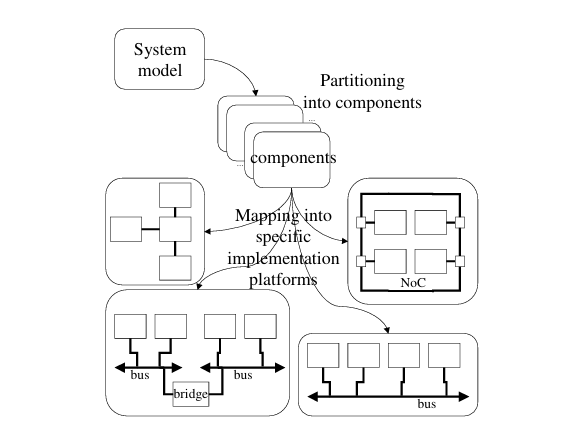
\includegraphics[width=0.6\textwidth]{Chapters/Figures/model_to_code_mapping.png}
  \caption{From models to code through model partitioning and mapping.}
  \label{fig:model_to_code_mapping}
\end{figure}

Conceptually, this design flow can be viewed in layers, as depicted in Figure~\ref{fig:model_to_code_mapping}:

\begin{itemize}
    \item \textbf{Top Layer: System Model Definition} \\
    At the top is the initial system model, which encapsulates the overall behavior, concurrency, and functional requirements of the embedded system. Within the context of this work, Input-Output Place-Transition (\gls{iopt}) Petri nets serve as the primary focus for this system-level specification \cite{iopttools, RefiningIOPT}. This model represents the complete, monolithic view of the controller logic before any distribution is considered.

    \item \textbf{Middle Layer:Component Identification via Decomposition} \\
    The holistic system model, as shown in Figure~\ref{fig:model_to_code_mapping}, is then subjected to partitioning, where it is divided into a set of distinct, concurrent components or sub-models. Each component typically reflects a specific functionality or a logically separable part of the overall system. Within the \gls{iopt}-Tools framework, this partitioning is achieved through formal net decomposition operations, such as net splitting (detailed in Section~\ref{sub:net_addicion}) \cite{Barrosadd, apresentacao}. This critical step transforms the single model into multiple \gls{iopt} sub-models, each representing a locally synchronous module designed to operate concurrently and interact with others. The "cutting sets" identified during decomposition define the logical interfaces and thus the necessary communication points between these emergent sub-models.

    \item \textbf{Bottom Layer: Component Mapping and Network Realization} \\
    Following decomposition, each sub-model (component) is mapped onto a specific implementation platform. These platforms can range from individual microcontrollers to dedicated processing units within a (\gls{fpga}), or even distinct software processes. As illustrated in Figure~\ref{fig:model_to_code_mapping}, the interaction between these distributed components must be realized through a defined network structure. The choice of network topology is essential and can have different variations, including:
    \begin{itemize}
        \item \textbf{Direct Connections:} Point-to-point links between two components, often suitable for dedicated, high-throughput, or low-latency communication.
        \item \textbf{Shared Buses:} Several components share a common communication channel, such as a "bus" or a "bridge"-connected "multi-bus" system (Figure~\ref{fig:model_to_code_mapping}), which necessitates mechanisms (e.g., communication protocols) for arbitration and addressing.
        \item \textbf{Network-on-Chip (NoC) Structures:} As depicted in Figure~\ref{fig:model_to_code_mapping}, NoCs provide more complex, scalable, and often packet-based communication fabrics integrated onto a single chip, suitable for systems with many interacting components.
    \end{itemize}
\end{itemize}

This layered approach directly correlates with the \textbf{GALS paradigm}. The decomposed \gls{iopt} sub-models from the middle layer naturally form the "Locally Synchronous" (LS) islands, each potentially operating within its own clock domain \cite{galsactd}. The communication between these locally  synchronous systems (or LS islands), facilitated by the network topologies defined at the bottom layer, is inherently asynchronous, realizing the "Globally Asynchronous" (GA) nature of the system \cite{galsborman}. \gls{iopt} nets extended with Asynchronous Channels (ACs) and Time Domains (TDs) are specifically designed to model such \gls{gals} systems, where ACs represent the logical communication pathways between components operating in different TDs \cite{galsactd, iopttools}.

The \textbf{IOPT net decomposition} (net splitting, Section~\ref{sub:net_addicion}) is thus a foundational step in this architectural mapping. It not only breaks down complexity but also explicitly defines the interfaces where inter-component communication is required. These interfaces, often realized as shared places or synchronized transitions in the original model, become the points where communication channels – logical at first, then physical – must be established \cite{Barrosadd}.

Finally, the selection of \textbf{communication protocols} (as detailed in Section~\ref{sec:communication_support_technologies}) is intrinsically linked to the chosen network topology and the characteristics of the \gls{gals} interactions. For instance:
\begin{itemize}
    \item Direct connections might be implemented using \gls{uart} for simple serial data exchange \cite{UARTwiki, Rao2021} or a dedicated \gls{fifo} with handshake logic for high-speed, reliable data streaming between two specific FPGAs or modules (as discussed in Section~\ref{sub:fifo+handshake}).
    \item Shared bus topologies, as illustrated in Figure~\ref{fig:model_to_code_mapping}, naturally lend themselves to protocols like I\textsuperscript{2}C, which includes addressing for multiple devices \cite{i2c,I2Cv2}, or \gls{spi}, where multiple slaves can be managed via individual select lines \cite{spisite, spisite2}.
    \item \gls{noc} architectures often employ more sophisticated packet-based protocols that handle routing, flow control, and error checking internally.
\end{itemize}
The communication channels modeled in the \gls{iopt} \gls{gals} framework, representing events or data exchange between sub-models, must be implemented using these protocols over the selected physical network. The design of the proposed automated code generation tool, central to this dissertation, aims to bridge the gap between the high-level specification of these decomposed \gls{iopt} sub-models and the concrete implementation of the communication logic using these diverse protocols and their underlying topological assumptions.





%%%%%%%%%%%%%%
%%%%%%%%%%%%%%
%%%%%%%%%%%%%%
%%%%%%%%%%%%%%
%%%%%%%%%%%%%%
		 %
		 %
		 %
		 %
		 %
%%%%%%%%%%%%%%
%%%%%%%%%%%%%%
%%%%%%%%%%%%%%
%%%%%%%%%%%%%%
%%%%%%%%%%%%%%



\section{IOPT tools}
\label{sec:iopt_tools}



The theoretical constructs of \gls{iopt} Petri nets (Section~\ref{sec:iopt_petri_nets}) and the principles of \gls{gals} architectures (Section~\ref{sec:gals}) find practical application in controller design through specialized software environments. One such comprehensive platform is \gls{iopt}-Tools, an integrated, web-based development environment tailored for the design, verification, and implementation of embedded system controllers, particularly for industrial automation and digital systems~\cite{iopttools}. As previously mentioned~\cite{iopttools}, \gls{iopt}-Tools supports a model-driven development workflow, starting from graphical Petri net model creation to verification and, crucially for this work, automatic code generation in C or \gls{vhdl}.

The environment's capacity to handle complex systems is partly due to its support for \gls{iopt} Petri net characteristics, including the input and output mechanisms essential for controller interaction and features facilitating model modularity, such as the net decomposition operations discussed in Section~\ref{sub:net_addicion}. These operations allow a complex controller model to be broken down into several distinct sub-models, which can then be targeted for execution on separate computational nodes, aligning with the distributed control paradigm.


In addition to design and verification, \gls{iopt}-Tools includes automatic code generation capabilities, enabling the creation of software in C or hardware descriptions in \gls{vhdl}~\cite{vhld}. This feature streamlines the transition from design to deployment, allowing for efficient and error-free implementation of the controller in either software or hardware~\cite{manual}.

\gls{iopt}-Tools delivers a complete, start-to-finish solution for creating controllers for embedded systems. The integration of graphical design, formal verification, and automatic code generation within a single, web-based platform significantly increases efficiency, reliability, and speed of controller development for both industrial and digital applications.


\subsection{Highlighting the Communication Gap}
\label{subsec:communication_gap}

While \gls{iopt}-Tools provides this extensive support for developing and generating code for individual controller logic, and facilitates the decomposition of models for distributed architectures, a significant challenge remains in automatically establishing and managing the communication between these distributed sub-models. The current automatic code generation primarily focuses on the internal logic of each individual sub-model. Crucially, it does not extend to automatically generating the necessary communication infrastructure required for these distinct sub-models to interact efficiently and reliably when deployed across different computational nodes.

This lack of automated support for different sub models, or petri nets, communication means that engineers must currently undertake the complex and error-prone task of manually implementing these communication links. This manual process involves selecting appropriate communication technologies (such as those reviewed in Section~\ref{sec:communication_support_technologies}), writing and integrating low-level driver code, and ensuring data consistency. This not only diminishes the benefits of automated generation for the core logic but also increases development time, hinders system optimization, and introduces potential for integration issues.

Addressing this specific gap,by designing and implementing a tool that automates the generation of code for efficient and reliable communication channels between distributed \gls{iopt} sub-models, is the central objective of this dissertation. This will further enhance \gls{iopt}-Tools' capabilities for developing truly distributed control systems.


\subsection{Overview of Key Components in IOPT-Tools}
\label{sub:iopt_tools_components}

A central component of the \gls{iopt}-Tools is its \textbf{graphical editor}, which facilitates the interactive design and modification of \gls{iopt} Petri net models directly within a standard web browser \cite{apresentacao}. This editor leverages \gls{ajax} principles, dynamically manipulating \gls{pnml} (Petri Net Markup Language) data in an \gls{xml} DOM document and utilizing XSL transformations to generate real-time \gls{svg} graphical representations. This architecture enables cross-platform compatibility and collaborative design, with features such as a persistent clipboard for inter-model data transfer and server-side sharing \cite{apresentacao}. The editor rigorously enforces \gls{iopt}-net syntactic rules and includes a specialized expression editor that guides users in constructing valid mathematical expressions for guard functions and output actions, thereby minimizing syntax errors \cite{apresentacao}.

For system verification and debugging, \gls{iopt}-Tools incorporates a robust \textbf{verification engine} primarily composed of a state-space generator and a query system \cite{manual, 2015gomes}. The state-space generator computes the reachability graph of an \gls{iopt} model, identifying potential design flaws such as deadlocks and transition conflicts. While state-space graphs can be extensive, the tool provides statistics and the option to view the graph for smaller models \cite{vhld}. To address the impracticality of visually inspecting large state-spaces, the query system allows users to define specific conditions based on net marking, output signals, and fired transitions. These queries are automatically checked during state-space computation, enabling automated model checking and property verification \cite{2015gomes}.

The framework also includes a \textbf{simulator tool} for executing and debugging \gls{iopt} models within the web browser \cite{2015gomes}. Distinct from traditional Petri net simulators, the \gls{iopt} simulator is designed for non-autonomous systems, allowing users to manipulate input signals and autonomous input events directly. It supports step-by-step and continuous execution with programmable speeds and breakpoints. A key feature is the automatic recording of simulation history, including net marking, signal values, and event triggers, which can be replayed, navigated, or exported for detailed analysis \cite{2015gomes}. The simulator employs a compilation execution strategy, dynamically generating JavaScript code for model semantics to ensure high performance \cite{2015gomes}.

Regarding \textbf{code generation}, \gls{iopt}-Tools offers automatic tools to produce C and \gls{vhdl} from \gls{iopt} models \cite{manual, vhld}. The C code generator produces ANSI C files suitable for microcontrollers or PCs, with the \texttt{net\_io.c} file requiring adaptation for specific hardware interfaces \cite{manual}. The \gls{vhdl} code generator synthesizes \gls{vhdl} component architectures, defining external interfaces based on \gls{iopt} signals and events, and handling internal logic for Petri net execution semantics \cite{vhld}. These generated components are synchronous, requiring input signals to be synchronized with a clock \cite{vhld}. While automatic code generation streamlines implementation and reduces low-level coding errors, the \gls{vhdl} generation, in particular, may incur a small penalty in resource consumption compared to expert-coded designs, though hardware vendor optimization tools are effective in mitigating this \cite{vhld}.However, while these generators effectively produce code for the internal logic of individual \gls{iopt} sub-models, they currently do not automatically generate the necessary communication infrastructure or low-level driver code required for these distinct sub-models to interact efficiently and reliably when deployed across different computational nodes.

Although not fully integrated into the main web interface at the time of some publications, other supplementary tools exist. These include SnoopyIOPT (an alternative editor), Split (essential for model decomposition into sub-models, as discussed in Section~\ref{sub:net_addicion}), Animator (for animated synoptics and GUIs), \gls{gui} Generator for \gls{fpga} (for \gls{gui} code from Animator), Configurator (for \gls{io} pin and hardware resource assignment), and HIPPO (for Petri net analysis and incidence matrix calculation) \cite{manual}. The potential for future integration of these tools into the web interface and the ongoing development of features like a waveform editor and in-circuit emulation highlight the continuous evolution of the \gls{iopt}-Tools framework \cite{2015gomes, manual}.





